\chapter{Attack Overview}
\label{chap:attack overview}
In this chapter, we first describe the attack and then specify the assumptions we make about the victim and the attacker.

\section{Attack Flow} First, a user preforms an action\footnote{\textbf{Action} is defined as a sequence of instruction related to a specific application to achieve a goal. Example: \texttt{addInsulin} is one possible action in the application DiabetesM. We consider that \texttt{opening} and \texttt{closing} applications are actions as well.} related to a targeted application on her smartwatch. This action triggers an encrypted Bluetooth communication between the smartwatch and its paired mobile phone. All this communication is captured by a local attacker. Finally, the attacker guesses which application generated the encrypted capture. Fig. \ref{fig:attack_overview} illustrates an overview of the attack.


\begin{figure}[H]
 \centering
 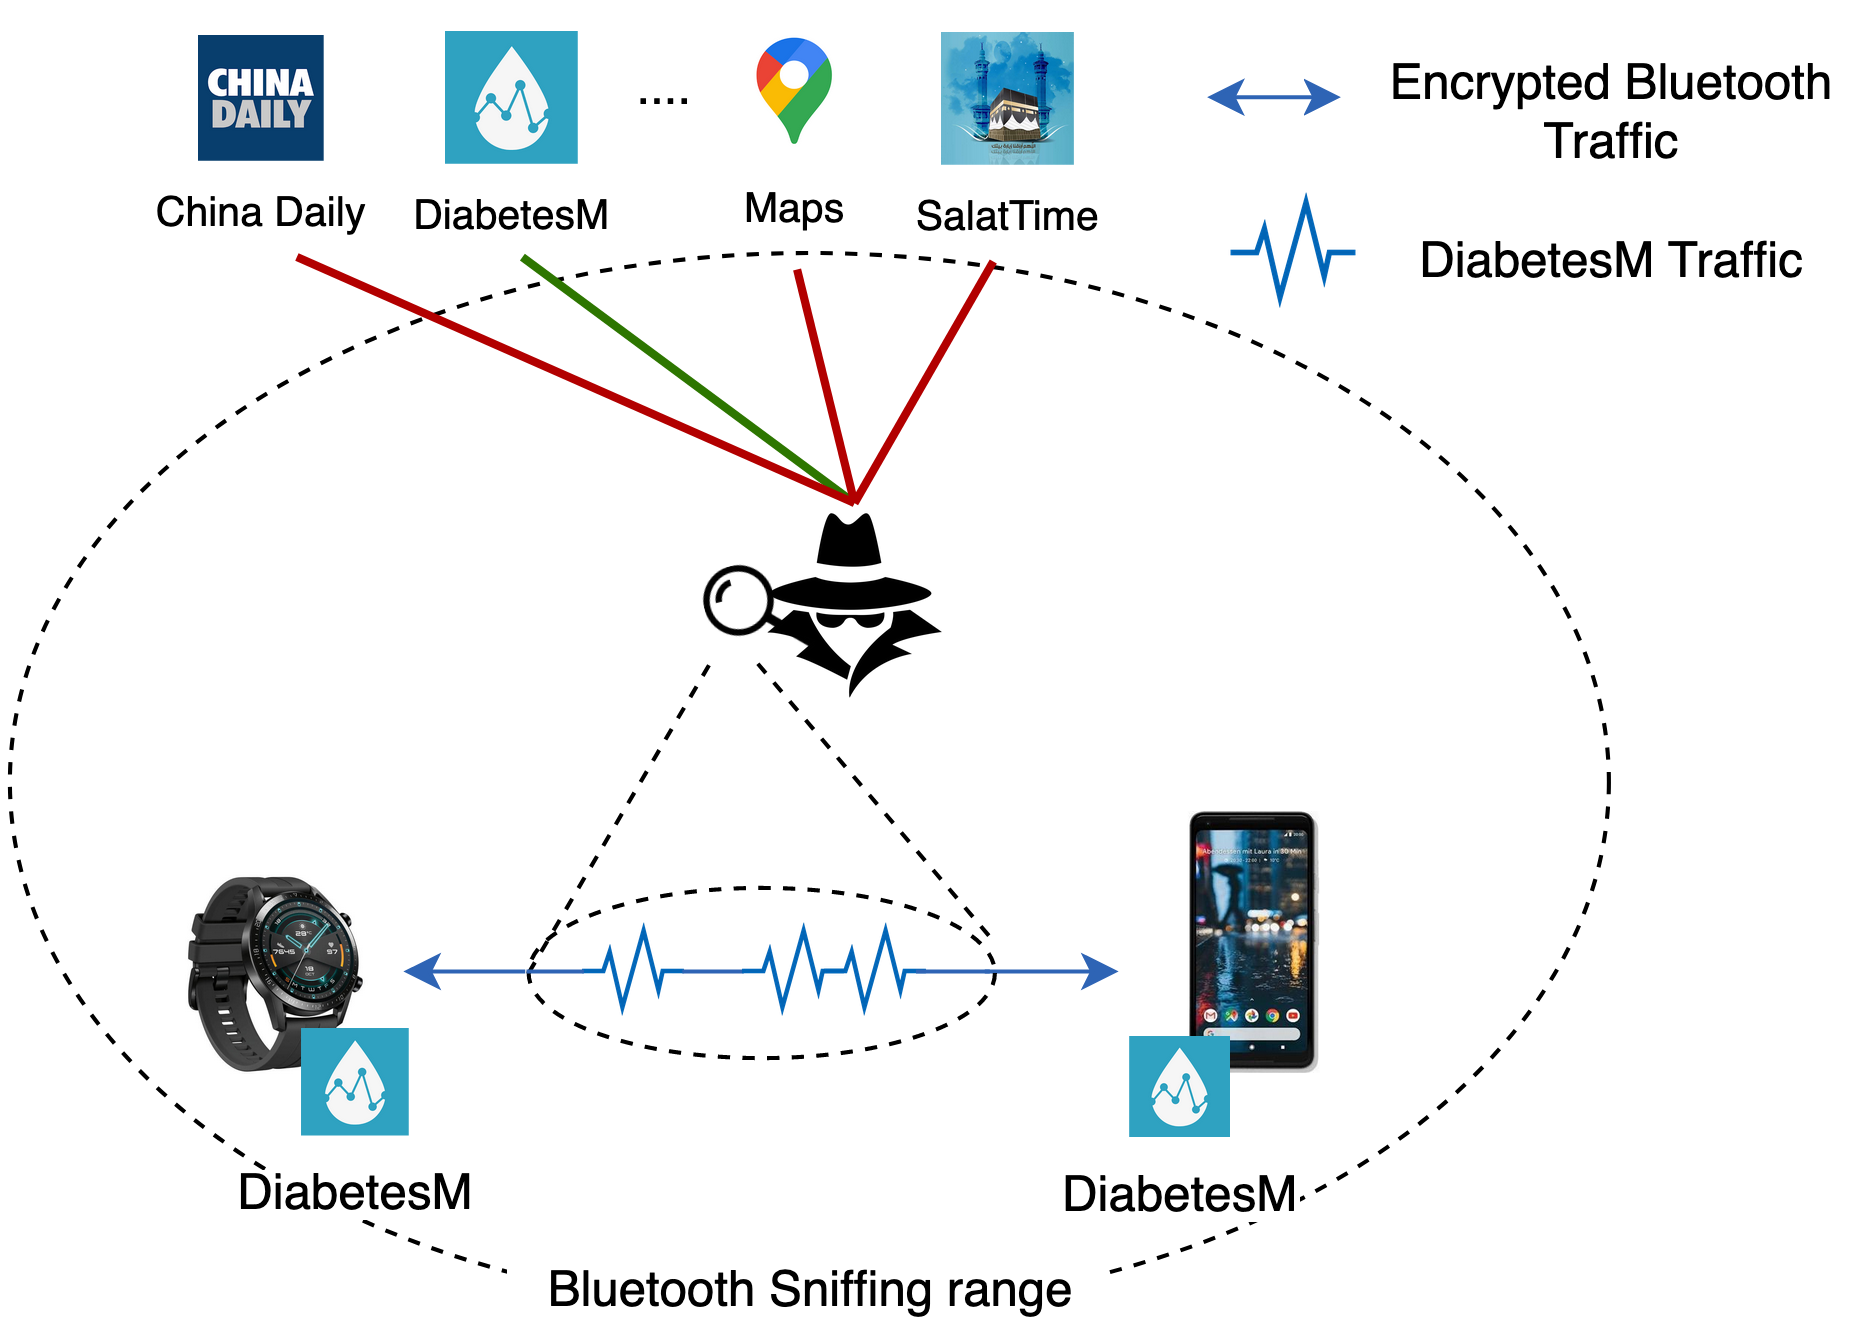
\includegraphics[width=0.8\textwidth]{figures/attack_overview.png}
 \caption[test]{Attack overview. An attacker is guessing correctly that the encrypted traffic recorded is from the Application DiabetesM\footnotemark}
 \label{fig:attack_overview}
\end{figure}
\footnotetext{\textbf{DiabetesM} is an application that helps diabetics to manage their diabetes.}


In Fig~\ref{fig:attack_overview}, the attacker is represented by a physical person. This can be the case if an attacker specifically follows a person to capture its Bluetooth traces with a portable sniffing device. However, we would more expect the attacker installing one or more sniffing devices at some location and coming from time to time to collect Bluetooth traces or directly transferring these traces to a remote server for a real-time analysis. 


\section{Threat Model} To summarize, we make the following assumptions regarding the attacker: 


\begin{enumerate}

    \item \textbf{Proximity}: The attacker is local to the victim.
    
    \item \textbf{The attacker is able to monitor the traffic}: The attacker possess the technology to monitor a targeted Bluetooth traffic.
    
    \item \textbf{Closed-World}: The victim is only using applications within a constrained set of applications which is known by the attacker.
    
    \item \textbf{Single-Action Capture}: The capture processed by the attacker contains only traffic related to a single action performed on the smartwatch.
    
    \item \textbf{Passive Attacker}: The attacker does not alter in anyway the communication between the victim's smartwatch and smartphone.
    
    \item \textbf{External Attacker} The attacker has no access to victim's phone or smartwatch. However, we assume that he has access to similar types of devices that he can buy.
    
    \item \textbf{The attacker cannot decrypt the traffic content}: We consider that the attacker is not able to decode the traffic. He deals only with encrypted traffic to infer information.
    
\end{enumerate}
\\
We saw in Sec.~\ref{sec:Bluetooth} that assumptions 1. and 2. can be adapted by the quality of the Bluetooth recorder and its antenna according to the attacker's budget. We minimize the impact of the \textit{Closed-World} assumption by leveraging the fact that for smartwatches the set of possible applications available for download is much more constrained than on smartphones, as discussed in Sec.~\ref{sec:smartwatches}. For the \textit{Single-Action} capture assumption, we extend our attack in Chapter~\ref{chap:towards_a_realistic_attack} to get rid of this assumption.
